\begin{IEEEbiography}[{\includegraphics[width=1in,height=1.25in,clip,keepaspectratio]{gsaponaro}}]{Giovanni Saponaro}
\end{IEEEbiography}

\begin{IEEEbiography}[{\includegraphics[width=1in,height=1.25in,clip,keepaspectratio]{lorenzo}}]{Lorenzo Jamone}
\end{IEEEbiography}

\begin{IEEEbiography}[{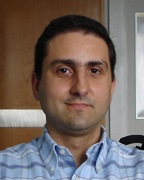
\includegraphics[width=1in,height=1.25in,clip,keepaspectratio]{./images/berna}}]{Alexandre Bernardino}
\end{IEEEbiography}

\begin{IEEEbiography}[{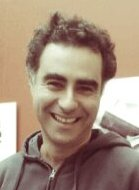
\includegraphics[width=1in,height=1.25in,clip,keepaspectratio]{./images/gsalvi}}]{Giampiero Salvi}
received the MSc degree in Electrical Engineering from Università la Sapienza (Rome, Italy) and the PhD degree in Computer Science from KTH Royal Institute of Technology (Stockholm, Sweden). He was a post-doctoral fellow at the Institute of Systems and Robotics (ISR), Lisbon, Portugal. He is currently Associate Professor in Machine Learning and Director of the Masters Programme in Machine Learning at KTH Royal Institute of Technology. His main interests are machine learning, speech technology, and cognitive systems.
\end{IEEEbiography}
